%\documentclass[11pt,oneside,a4paper,openright]{report}
%\usepackage[utf8]{inputenc}
%\renewcommand{\contentsname}{Indholdsfortegnelse}
%\usepackage{pdfpages}
%\usepackage{titlesec}
%\titleformat{\chapter}{\normalfont\huge}{\thechapter.}{20pt}{\huge\it}

%%%% Dokumentklassen %%%%

\documentclass[a4paper,11pt,dvipsnames,oneside,openany]{memoir} 	% Openright åbner kapitler på højresider (openany begge)
% fleqn = flush left equation - sikre at alle ligninger tvinges til venstre. I 3. semesterprojektet, skulle ligningerne stå i midten derfor er denne pakke slettet fra dokumentklassen.

\usepackage{subfiles}
\usepackage{nameref}
\usepackage{tabularx}
\usepackage{multirow}
\usepackage[table]{xcolor}


%%%% PACKAGES %%%%

%% Oversættelse og tegnsætning %%
\usepackage[utf8]{inputenc}					% Input-indkodning af tegnsæt (UTF8)
\usepackage[danish]{babel}					% Dokumentets sprog
\usepackage[T1]{fontenc}				    % Output-indkodning af tegnsæt (T1)
\usepackage{ragged2e,anyfontsize}			% Justering af elementer
%\usepackage{fixltx2e}						% Retter forskellige fejl i LaTeX-kernen
\usepackage{titletoc}
\newcommand{\nocontentsline}[3]{}
\newcommand{\tocless}[2]{\bgroup\let\addcontentsline=\nocontentsline#1{#2}\egroup}									% Giver mulighed for at fjerne section nummer i indholdsfortegnelse ved \tocless


\usepackage{lastpage}						% Total antal sider opdateres automatisk ved \pageref{LastPage}
\usepackage{tikz}							% Til at lave flow diagrammer
\usetikzlibrary{calc,trees,positioning,arrows,chains,shapes.geometric,decorations.pathreplacing,decorations.pathmorphing,shapes,matrix,shapes.symbols}				% Til at lave diagrammer
																			
%% Figurer og tabeller (floats) %%
\usepackage{graphicx} 						% Håndtering af eksterne billeder (JPG, PNG, EPS, PDF)
\usepackage{multicol}         	           	% Muliggør output i spalter
\usepackage{rotating}						% Rotation af tekst med \begin{sideways}...\end{sideways}
\usepackage{xcolor}							% Definer farver med \definecolor. Se mere: http://en.wikibooks.org/wiki/LaTeX/Colors
\usepackage{flafter}						% Sørger for at floats ikke optræder i teksten før deres reference
\let\newfloat\relax 						% Justering mellem float-pakken og memoir
\usepackage{float}							% Muliggør eksakt placering af floats, f.eks. \begin{figure}[H]
\usepackage{color, colortbl}				% Tilføjer farve til tabeller

\definecolor{Gray}{gray}{0.9}				% Definerer en farve "yeezy-gray"

%% Matematik mm. %%
\usepackage{amsmath,amssymb,stmaryrd} 		% Avancerede matematik-udvidelser
\usepackage{mathtools}						% Andre matematik- og tegnudvidelser
\usepackage{textcomp}                 		% Symbol-udvidelser (fx promille-tegn med \textperthousand)
\usepackage{rsphrase}						% Kemi-pakke til RS-saetninger, fx \rsphrase{R1}
\usepackage[version=3]{mhchem} 				% Kemi-pakke til flot og let notation af formler, f.eks. \ce{Fe2O3}
\usepackage{siunitx}						% Flot og konsistent præsentation af tal og enheder med \si{enhed} og \SI{tal}{enhed}
\sisetup{output-decimal-marker = {,}}		% Opsætning af \SI (DE for komma som decimalseparator) 

%% Referencer og kilder %%
\usepackage[danish]{varioref}				% Muliggør bl.a. krydshenvisninger med sidetal (\vref)
\usepackage{natbib}							% Udvidelse med naturvidenskabelige citationsmodeller
\usepackage{xr}							    % Referencer til eksternt dokument med \externaldocument{<NAVN>}

%% Misc. %%
\usepackage{listings}						% Placer kildekode i dokumentet med \begin{lstlisting}...\end{lstlisting}
\usepackage{lipsum}							% Dummy text \lipsum[..]
\usepackage[shortlabels]{enumitem}			% Muliggør enkelt konfiguration af lister
\usepackage{pdfpages}						% Gør det muligt at inkludere pdf-dokumenter med kommandoen \includepdf[pages={x-y}]{fil.pdf}	
\pdfoptionpdfminorversion=6					% Muliggør inkludering af pdf-dokumenter, af version 1.6 og højere
\pretolerance=2500 							% Justering af afstand mellem ord (højt tal, mindre orddeling og mere luft mellem ord)


%%%% CUSTOM SETTINGS %%%%

%% Marginer %%
\setlrmarginsandblock{3.0cm}{3.0cm}{*}		% \setlrmarginsandblock{Indbinding}{Kant}{Ratio}
\setulmarginsandblock{3.0cm}{3.0cm}{*}		% \setulmarginsandblock{Top}{Bund}{Ratio}
\checkandfixthelayout 						% Oversætter værdier til brug for andre pakker

%% Afsnitsformatering %%
\setlength{\parindent}{0mm}           		% Størrelse af indryk
\setlength{\parskip}{3mm}          			% Afstand mellem afsnit ved brug af double Enter
\linespread{1,1}							% Linjeafstand

%% Indholdsfortegnelse %%
\setsecnumdepth{subsection}		 			% Dybden af nummererede overskrifter (part/chapter/section/subsection)
\maxsecnumdepth{subsection}					% Dokumentklassens grænse for nummereringsdybde
\settocdepth{subsubsection} 					% Dybden af indholdsfortegnelsen
\setcounter{secnumdepth}{5} 				    % Ekstra subsubsection nummerering
		
%% Opsætning af listings %%
\definecolor{commentGreen}{RGB}{34,139,24}
\definecolor{stringPurple}{RGB}{208,76,239}

\lstset{language=Matlab,				    % Sprog
	basicstyle=\ttfamily\scriptsize,	    % Opsætning af teksten
	keywords={for,if,while,else,elseif,		% Nøgleord at fremhæve
			  end,break,return,case,
			  switch,function},
	keywordstyle=\color{blue},				% Opsætning af nøgleord
	commentstyle=\color{commentGreen},		% Opsætning af kommentarer
	stringstyle=\color{stringPurple},		% Opsætning af strenge
	showstringspaces=false,					% Mellemrum i strenge enten vist eller blanke
	numbers=left, numberstyle=\tiny,		    % Linjenumre
	extendedchars=true, 					    % Tillader specielle karakterer
	columns=flexible,						% Kolonnejustering
	breaklines, breakatwhitespace=true,		% Bryd lange linjer
}

%% Navngivning %%
\addto\captionsdanish{
	\renewcommand\appendixname{Appendiks}
	\renewcommand\contentsname{Indholdsfortegnelse}	
	\renewcommand\appendixpagename{Appendiks}
	\renewcommand\appendixtocname{Appendiks}
	\renewcommand\cftchaptername{\chaptername~}		% Skriver "Kapitel" foran kapitlerne i indholdsfortegnelsen
	\renewcommand\cftappendixname{\appendixname~}	% Skriver "Appendiks" foran appendiks i indholdsfortegnelsen
}

%% Kapiteludssende %%
\definecolor{numbercolor}{gray}{0.7}		            % Definerer en farve til brug til kapiteludseende
\newif\ifchapternonum

\makechapterstyle{jenor}{					        % Definerer kapiteludseende frem til ...
  \renewcommand\beforechapskip{0pt}
  \renewcommand\printchaptername{}
  \renewcommand\printchapternum{}
  \renewcommand\printchapternonum{\chapternonumtrue}
  \renewcommand\chaptitlefont{\fontfamily{pbk}\fontseries{db}\fontshape{n}\fontsize{25}{35}\selectfont\raggedleft}
  \renewcommand\chapnumfont{\fontfamily{pbk}\fontseries{m}\fontshape{n}\fontsize{1in}{0in}\selectfont\color{numbercolor}}
  \renewcommand\printchaptertitle[1]{%
    \noindent
    \ifchapternonum
    \begin{tabularx}{\textwidth}{X}
    {\let\\\newline\chaptitlefont ##1\par} 
    \end{tabularx}
    \par\vskip-2.5mm\hrule
    \else
    \begin{tabularx}{\textwidth}{Xl}
    {\parbox[b]{\linewidth}{\chaptitlefont ##1}} & \raisebox{-15pt}{\chapnumfont \thechapter}
    \end{tabularx}
    \par\vskip2mm\hrule
    \fi
  }
}											        % ... her

\chapterstyle{jenor}						        % Valg af kapiteludseende - Google 'memoir chapter styles' for alternativer

%% Sidehoved %%

\makepagestyle{AAU}							        % Definerer sidehoved og sidefod udseende frem til ...
\makepsmarks{AAU}{%
	\createmark{chapter}{left}{shownumber}{}{. \ }
	\createmark{section}{right}{shownumber}{}{. \ }
	\createplainmark{toc}{both}{\contentsname}
	\createplainmark{lof}{both}{\listfigurename}
	\createplainmark{lot}{both}{\listtablename}
	\createplainmark{bib}{both}{\bibname}
	\createplainmark{index}{both}{\indexname}
	\createplainmark{glossary}{both}{\glossaryname}
}
\nouppercaseheads									% Ingen Caps ønskes

\makeevenhead{AAU}{\small E17BAC-Synk2}{}{\leftmark}	% Definerer lige siders sidehoved (\makeevenhead{Navn}{Venstre}{Center}{Hoejre})
\makeoddhead{AAU}{\rightmark}{}{}		            % Definerer ulige siders sidehoved (\makeoddhead{Navn}{Venstre}{Center}{Højre})
\makeevenfoot{AAU}{\small \thepage \ }{}{ }						% Definerer lige siders sidefod (\makeevenfoot{Navn}{Venstre}{Center}{Højre})
\makeoddfoot{AAU}{}{}{\small \thepage \ }						% Definerer ulige siders sidefod (\makeoddfoot{Navn}{Venstre}{Center}{Højre})

\copypagestyle{AAUchap}{AAU}							% Sidehoved for kapitelsider defineres som standardsider, men med blank sidehoved
\makeoddhead{AAUchap}{}{}{}
\makeevenhead{AAUchap}{}{}{}
\makeheadrule{AAUchap}{\textwidth}{0pt}
\aliaspagestyle{chapter}{AAUchap}					% Den ny style vælges til at gælde for chapters
													% ... her
															
\pagestyle{AAU}										% Valg af sidehoved og sidefod


%%%% CUSTOM COMMANDS %%%%

%% Billede hack %%
\newcommand{\figur}[4]{
		\begin{figure}[H] \centering
			\includegraphics[width=#1\textwidth]{billeder/#2}
			\caption{#3}\label{#4}
		\end{figure} 
}

%% Specielle tegn %%
\newcommand{\decC}{^{\circ}\text{C}}
\newcommand{\dec}{^{\circ}}
\newcommand{\m}{\cdot}


%%%% ORDDELING %%%%

\hyphenation{}


%%%% Tilføjelser af min preample %%%%

% Booktabs:
% The booktabs package is needed for better looking tables. 
\usepackage{booktabs}

% Caption:
% For better looking captions. See caption documentation on how to change the format of the captions.
\usepackage[hang, font={small, it}]{caption}

% Hyperref:
% This package makes all references within your document clickable. By default, these references will become boxed and colored. This is turned back to normal with the \hypersetup command below.
\usepackage{hyperref}
	\hypersetup{colorlinks=false,pdfborder=0 0 0}

% Cleveref:
% This package automatically detects the type of reference (equation, table, etc.) when the \cref{} command is used. It then adds a word in front of the reference, i.e. Fig. in front of a reference to a figure. With the \crefname{}{}{} command, these words may be changed.
\usepackage{cleveref}
	\crefname{equation}{formel}{formler}
	\crefname{figure}{figur}{figurer}	
	\crefname{table}{tabel}{tabeller}

% Mine tilføjelser:
\usepackage{units}                        %% Bruges til at gøre fx 1/2 samlet med: \nicefrac{1}{2}.
\usepackage{tabu, longtable}              %% Bruges til tabeller.
\setlength{\tabulinesep}{1.5ex}           %% Definerer linjeafstand i tabeller.
\usepackage{enumerate}                    %% Bruges til lister.
\usepackage{tabto}                        %% Giver mulighed for TAB med fx \tabto{3em}.
\usepackage[hyphenbreaks]{breakurl}       %% Bruges til websiders url'er.
\renewcommand{\UrlFont}{                  %% Definerer url-font.
\small\ttfamily}                          %
\bibliographystyle{unsrt}                 %% Definere bibliografien. Ses til sidst i dokumentet i kapitlet Litteratur.
\usepackage{amssymb} 
\usepackage{pifont}
%\newcommand{\xmark{\ding{55}}			 % Opretter et unchecked mark

\usepackage[bottom]{footmisc}

\usetikzlibrary{%
    decorations.pathreplacing,%
    decorations.pathmorphing,%
    arrows,
    arrows.meta,
    positioning,
    shapes,
    shadows,
    shapes.geometric
    }
    \usepackage{relsize}

%\definecolor{myblue1}{RGB}{0,157,209}
\definecolor{myblue1}{rgb}{0.12, 0.56, 1.0}
\definecolor{myblue3}{RGB}{216,229,245}
%\definecolor{myblue4}{RGB}{0,149,229}
\definecolor{myblue2}{rgb}{0.19, 0.55, 0.91}
\definecolor{myblue4}{rgb}{0.08, 0.38, 0.74}
\definecolor{myred1}{rgb}{0.82, 0.1, 0.26}
\definecolor{myyellow1}{rgb}{1.0, 0.96, 0.0}
\definecolor{myyellow2}{rgb}{1.0, 0.65, 0.0}


\usepackage{pdflscape}
\usepackage{rotating}


\begin{document}

\begin{titlingpage}
\begin{center}

~ \\[3cm]

%\includegraphics[width=0.6\textwidth]{figurer/ASE}~\\[1cm]

\textsc{\LARGE Bilag 4}\\[1.5cm]

%\textsc{\Large Sundhedsteknologi}\\
%\textsc{\Large 3. semesterprojekt}\\[0.5cm]

\noindent\makebox[\linewidth]{\rule{\textwidth}{0.4pt}}\\
[0.5cm]{\Huge Analyse}
\noindent\makebox[\linewidth]{\rule{\textwidth}{0.4pt}}
\end{center}
\vfill
\begin{center}
{\large 19. december 2017}
\end{center}
\end{titlingpage}



\newpage
\tableofcontents*
\newpage
\chapter{Ordliste}

\begin{longtabu} to \linewidth{@{}l X[j]@{}}
    Ord &    Forklaring\\
    \toprule \
   BI 	&    Bioimpedans \\
    
 
\label{forkort}
\end{longtabu}

\chapter{Indledning}

I dette bilag vil der blive beskrevet de overvejelser om mulige løsninger i projektet og hvilke der er valgt at gå videre med udgangspunkt i artiklen \textit{"Bioimpedance Analysis: A Guide to Simple Design and Implementation"}. I de følgende afsnit er der beskrevet og diskuteret valget af hardware- og software komponenter som er kritiske for det ønsket system. I artiklen er der givet et kredsløb som kan ses på figur \ref{fig:BIdiagram}, som repræsenterer en simple BI-måler, der består af en instrumenteringsforstærker, en strømgenerator og to elektroder. Kredsløbet fungerer ved at funktionsgeneratoren genererer et AC signal, som sendes til en strømgenerator, som på baggrund af det indsendte signal genererer en kendt konstant strøm. Denne kendte strøm sendes til et måleobjekt igennem to elektroder. Ved at måle spændingsfaldet over elektroderne, kan man regne måleobjektets impedans vha. af ohms lov: $$R=\frac{V}{I}$$

Det er denne BI-måler der vil blive realiseret, bygget på et fumlebræt og testet. Der er indkøbt præcist de komponenter som der bruges i kredsløbet, dog udstyr som oscilloskop og A/D-konverter vil der blive brugt kendt udstyr for projektgruppen. 






\begin{figure}[H]
\centering
{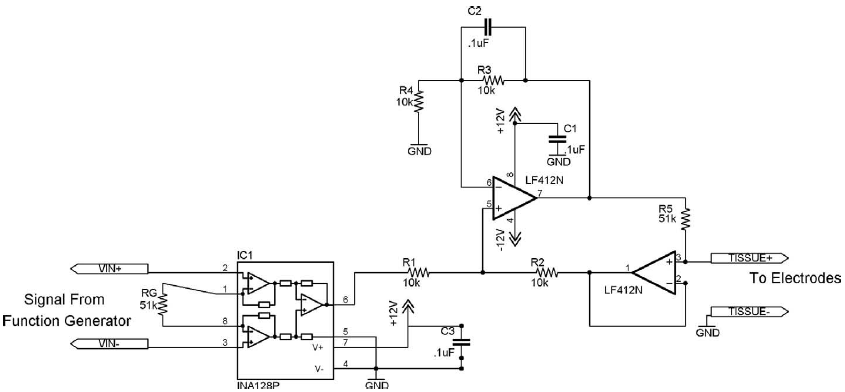
\includegraphics[width=12cm]
{Figure/BIdiagram}}
\caption{Diagram over det oprindelige kredsløb\cite{Aroom2009}}
\label{fig:BIdiagram}
\end{figure}


\chapter{Bioimpedans}
\section{Introduktion}
BI er en ikke invasiv målemetode som er billig, simpel og hurtig at udføre. Når man måler BI bruges der elektroder som kan placeres der hvor man ønsker at måle. Enten hele kroppen eller en bestem kropssegment. Målingen består af to sæt elektroder. Det ene par elektroder sender en uskadelig AC strøm i uA og et andet måler spændingsfaldet over vævet. Impedansen i vævet varierer fra væv til væv. Hvor væske og elektrolytter har en høj ledningsevne, giver en lav impedans og hvorimod fedt og knogler har en lav ledningsevne giver en høj impedans.\cite{Brantlov2017} 

Det biologisk vævs celler kan vises som en model som består af tre elektriske komponenter. Ekstracellulærvæsken, intracellulærvæsken og cellemembranen. Ekstracellulærvæsken er repræcenteret som en modstand parallelt med intracellulærvæsken og cellemembranen. Intracellulærvæsken består af en modstand og cellemembranen som en kondensator som vist i figur \ref{fig:vaevsmodel}.

\begin{figure}[H]
\centering
{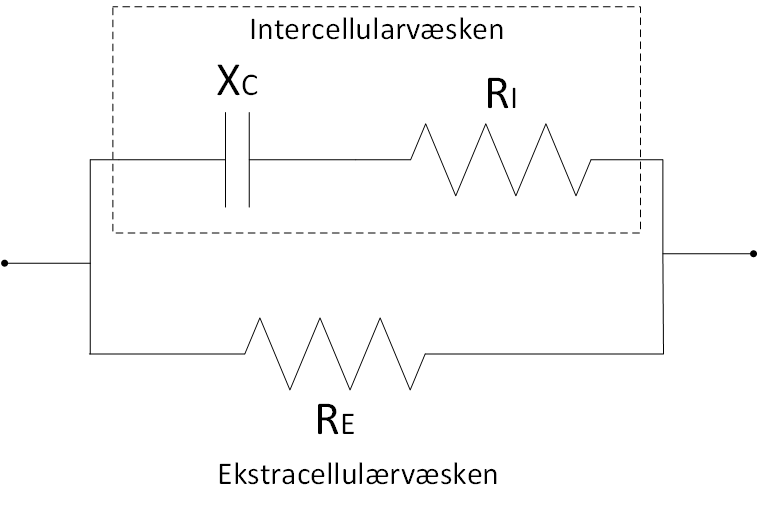
\includegraphics[width=10cm]
{Figure/vaevsmodel}}
\caption{Biologisk cellemodel som elektrisk kredsløb. En del af kredsløbet er relateret til dobbeltlaget i cellemembranen og intercellularvæsken, hvor X\textsubscript{C} har kapacitive egenskaber og R\textsubscript{I} er modstanden i intercellularvæsken. Den anden del er relateret til ekstracellulærvæsken, R\textsubscript{E} som er modstanden i ekstracellulærvæsken.}
\label{fig:vaevsmodel}
\end{figure}

Forholdet i mellem i cellemodellen kan blive illustreret ved at plotte Z som en vektor i et koordinatsystem fra (0,0) til R\textsubscript{I}X\textsubscript{C}. Værdien af Z er længden af vektoren beregnet med formlen: 
\begin{equation}
Z=\sqrt{R^{2}+X^{2}_{C}}
\end{equation} 

\begin{figure}[H]
\centering
{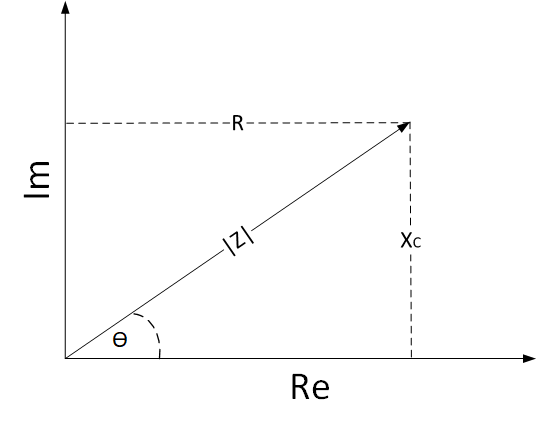
\includegraphics[width=10cm]
{Figure/vektor}}
\caption{Forholdet imellem den kapacitive reaktans (X\textsubscript{C}), modstanden (R), impedansen (Z) og fasen vinklen ($\theta$) i grader.}
\label{fig:vektor}
\end{figure}


Når impedansen måles på et biologisk væv er frekvensen afgørende for resultatet af impedansen, da denne vil opføre sig forskelligt afhængig af frekvensen. Ved en lav frekvens på under 100 Hz løber strømmen i ekstracellulærvæsken, så den totale impedans er mere resistiv og svare mere til ekstracellulærvæsken. Som i figur \ref{fig:celler} kan det ses at membranen rundt om cellen sørger for at der ikke kan passerer lav frekvent strøm (rød) igennem cellen. Ved højere frekvens er det muligt at bryde membranen og trænge igennem cellen (blå). Ved den høje frekvens er der nu adgang til elektriske ioner i både ekstracellulærvæsken og intracellulærvæsken hvilket giver en lavere impedans. 

%Den tilførte strøm der løber igennem vævet løber også igennem vævets celler. Da cellerne indeholder intracellulærvæske og ekstracellulærvæske vil den denne strøm opføre sig forskelligt ved lave og høje frekvenser. Hvor ved lave frekvenser kan strømmen kun trænge igennem ekstracellulærvæsken, hvor ved høje frekvenser kan strømmen trænge igennem både intracellulærvæsken og ekstracellulærvæsken i cellen. 

\begin{figure}[H]
\centering
{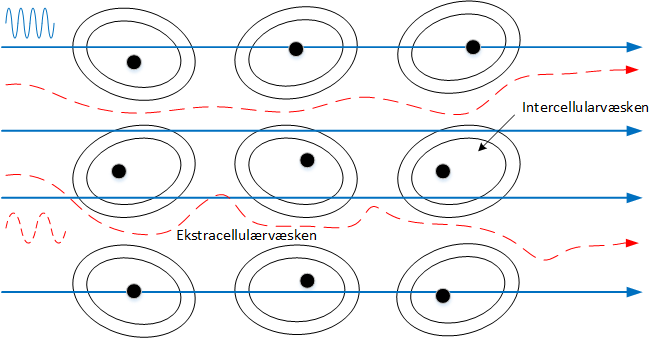
\includegraphics[width=10cm]
{Figure/celler}}
\caption{}
\label{fig:celler}
\end{figure}



%BI måles ved at der bliver tilført strøm over et område, hvor på man måler spændningen over. 

%\begin{figure}[H]
%\centering
%{\includegraphics[width=10cm]
%{Figure/BIbasic}}
%\caption{}
%\label{fig:BIbasic}
%\end{figure}






\section{Opbygning af BI-måler}
Princippet i at måle BI er ved at tilføre en strøm over vævet med elektroder, hvor på man måler spændingen over elektroderne. Dette princip bliver omtalt i artikel \citep{Aroom2009} hvor der er en beskrivelse af et prisbilligt kredsløb som kan måle BI. Der er diagrammer med komponentværdier som vil være et udgangspunkt for udviklingen af bioimpedans måleren. Der vil i de følgende afsnit blive gennemgået opbygningen af BI-måleren fra artikelen og til slut realiseret, testet op imod dokumentation fra artiklen og om der kan detekteres et synk. 



\section{Hardware}

Overordnet bestod det samlet system af BI-måleren som vist i blokke i figur \ref{fig:oprindeligebd}. Hvor det var muligt, blev komponenter inden de blev monteret på fumlebræt, først testet i simuleringsværtøjet Multisim. Her var det muligt at se om de fungerede som ønsket. I de følgende afsnit vil disse blokke blive beskrevet nærmere. 

\begin{figure}[H]
\centering
{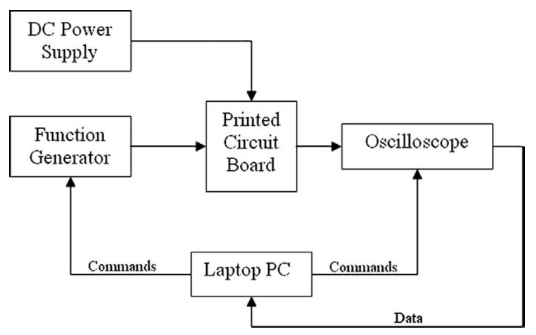
\includegraphics[width=10cm]
{Figure/oprindeligebd}}
\caption{Blokdiagram over det oprindelige kredsløb\cite{Aroom2009}}
\label{fig:oprindeligebd}
\end{figure}

\subsection{Strømforsyning}
I artiklen \citep{Aroom2009}  blev der brugt en $\pm$12 V strømforsyning tilsluttet til netforsyningen. For at undgå netforsyningen blev der i stedet for brugt almindelige AA batterier. For at bruge samme forsyningsspænding blev der valgt at sætte otte AA batterier i serie, som i figur \ref{fig:12vbatteri}, nu var det muligt at have en forsyning på +12 V og -12 V kun med batterier. Batterierne blev også valgt da de var nemt tilgængelige og fordi der ikke var nogle kritiske komponenter som var afhængige af en fast og præcis spænding som kunne resulterer i fejlmålinger BI-måleren. 

\begin{figure}[H]
\centering
{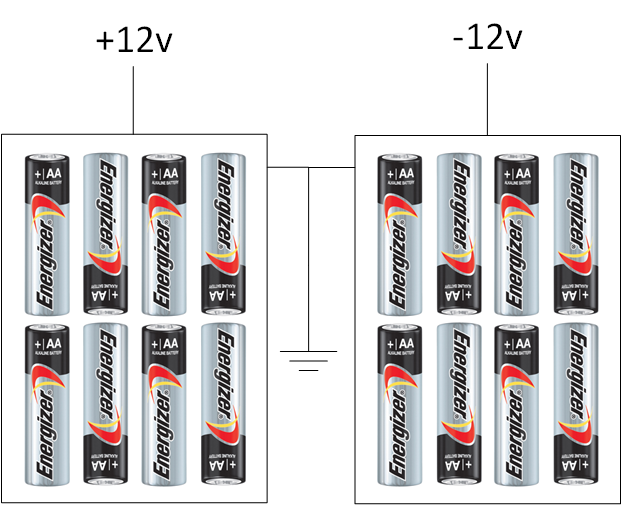
\includegraphics[width=10cm]
{Figure/12vbatteri}}
\caption{2x8 batterier sat sammen gav mulighed for at have en forsyning på $\pm$12 v, for at undgå at få stød fra netforsyningen.}
\label{fig:12vbatteri}
\end{figure}

\subsection{Funktionsgenerator}
Funktionsgeneratoren funktion var at sende en fast frekvens ind i kroppen og samtidig en fast spænding til strømgeneratoren. 
Analog Discovery tilsluttet en PC, blev brugt som funktionsgenerator, forbundet som på figur \ref{fig:analogdis}, da denne er nem og hurtig til at generere signaler. Den ønskede frekvens på 50 kHz blev brugt, da det er en brugt frekvens når der skal måles et synk\cite{Kusuhara2004} \citep{Brantlov2017}. Amplituden blev sat til 2 V. 

\begin{figure}[H]
\centering
{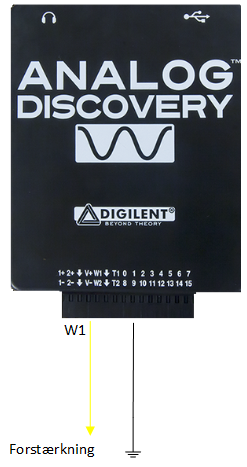
\includegraphics[width=4cm]
{Figure/analogdis}}
\caption{Diagram over hvilke porte på Analog discovery der blev brugt  som funktionsgenerator. Waveform 1 som går videre til instrumentationsforsærkeren og ground som går til stel på fumlebrættet}
\label{fig:analogdis}
\end{figure}


\subsection{Forstærkning}
Signalet fra Analog Discovery gik ind til instrumentationsforstærkeren INA128 som der også blev brugt i artiklen. Figure \ref{fig:ina128} viser diagram over INA128, hvor den tilhørende gain modstand (R\textsubscript{G}) på 51 kohm blev også brugt, da det gav en fordobling i forstærkning, ved opslag i datablad. På udgangen af INA128 var der nu 4V. Fordelene ved instrumentationsforstærkeren, udover at forstærke signalet, kan der nævnes\cite{PeterJohansen2014}:

\begin{itemize}
\item Reducer common-mode støj
\item Differentielt input
\item gain justering med kun en modstand
\end{itemize}


\begin{figure}[H]
\centering
{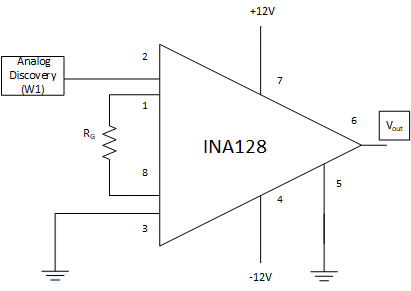
\includegraphics[width=10cm]
{Figure/ina128}}
\caption{Diagram over INA128 med differentielt input. Hvor den ene indgang (ben 2) var forbundet med Analog Discovery og (ben 3) forbundet til stel. Gain modstand (R\textsubscript{G} på 51 kohm. Eksitastionsspændingen på $\pm$12 V. Udover var stel (ben 5) kom det forstærket signal ud (ben 6).  }
\label{fig:ina128}
\end{figure}


\begin{figure}[H]
\centering
{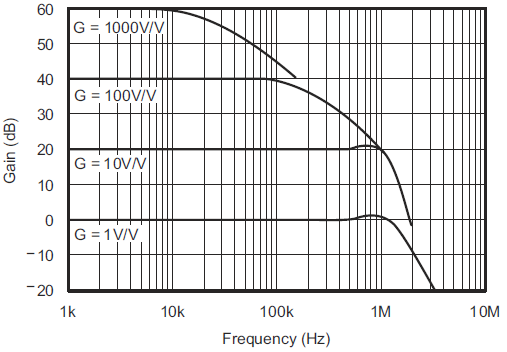
\includegraphics[width=10cm]
{Figure/ina128gain}}
\caption{Oversigt fra INA128 datablad over hvilke maks frekvenser INA128 kan arbejde indenfor ved bestemte gains.}
\label{fig:ina128gain}
\end{figure}

Ved en gain på 2 (V/V) kan der aflæses i figur \ref{fig:ina128gain} som er fra databladet til INA128, at båndbredden var over 100 kHz, hvilket er indenfor den ønskede frekvens på 50 kHz og at INA128 ikke er belastet på nogle måde. 

\subsection{Strømgenerator}

Spændningen på 2 V kommer ind ved modstand R1 og strømmen ud ad ben 3 på LF412N. Kombinationen af bestemt ohmsk modstand størrelse og lav \% tolerance modstand giver den faste strøm. Her er der brugt 1\% modstande. Ved at ændre modstand R5, kan en ønsket strøm beregnes vha. formlen\cite{Aroom2009}: $$I_{tissue}=2*\frac{V_{in}}{R_{5}}$$


\begin{figure}[H]
\centering
{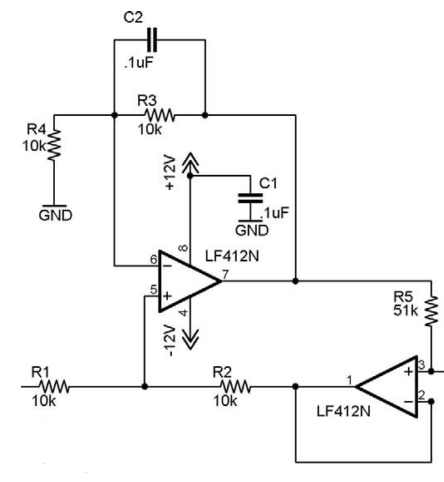
\includegraphics[width=10cm]
{Figure/howland1}}
\caption{Diagram over VCCS som er bygget op efter Howland princippet. Den faste spænding på 4V til VCCS giver en fast strøm på 23uA ved 50kHz.}
\label{fig:howland1}
\end{figure}




\subsection{Elektroder}

\begin{figure}[H]
\centering
{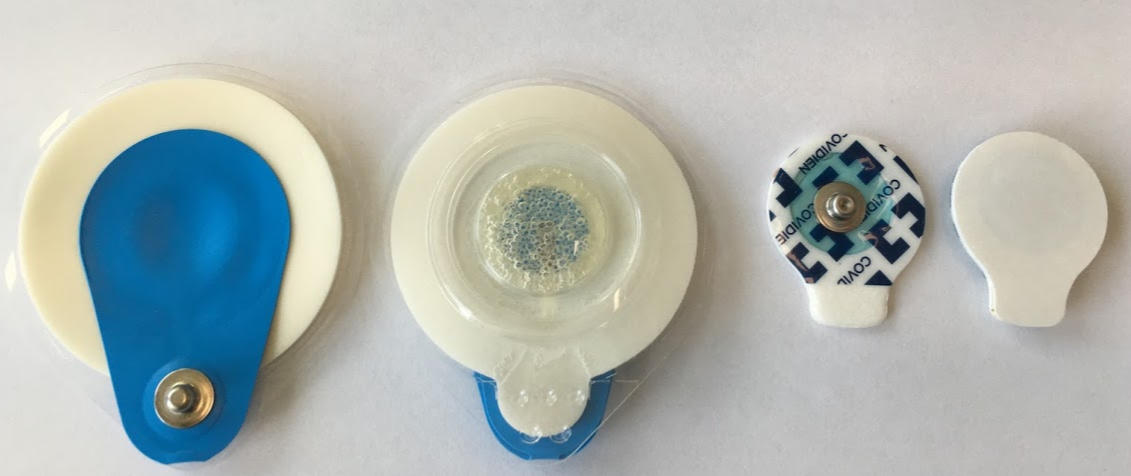
\includegraphics[width=12cm]
{Figure/elektroder}}
\caption{Ved målingerne er der blevet brugt EKG elektroder (venstre) og EMG elektroder (højre).}
\label{fig:elektroder}
\end{figure}

De forskellige elektroder kan ses i figur \ref{fig:elektroder}. EKG elektroderne er nemme at påsætte og indeholder meget gel som giver optimal kontakt, men fysisk fylder de meget. EMG elektroderne har mindre gel, men fylder næsten ingen ting. Der blev prøvet forskellige placeringer til elektroderne men brugte artikel \cite{Nahrstaedt2012a} som vejledende placering \ref{fig:elektrodeplaceringREF}. 


\begin{figure}[H]
\centering
{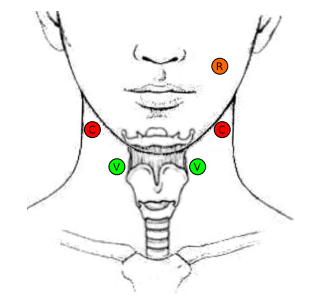
\includegraphics[width=8cm]
{Figure/elektrodeplaceringREF}}
\caption{Placering af elektroderne som blev brugt til vejledning\cite{Nahrstaedt2012a}}
\label{fig:elektrodeplaceringREF}
\end{figure}





\subsection{A/D-konverter}

Analog Discovery er tilsluttet en pc via USB og det analogt signal blev samplet ved at måle over elektroderne. Der blev også monteret et multimeter i serie for at aflæse den konstante strøm.


\begin{figure}[H]
\centering
{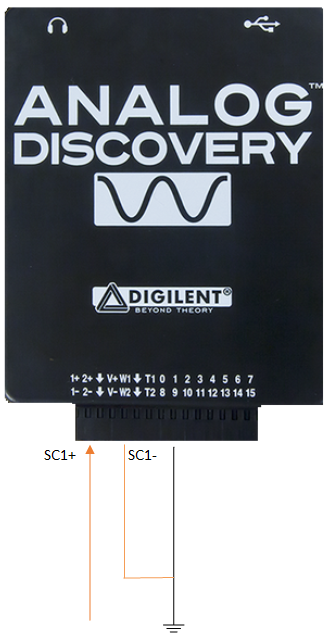
\includegraphics[width=6cm]
{Figure/adkonverter}}
\caption{Scope channel 1 positiv blev brugt til at måle spændingen over elektroderne}
\label{fig:adkonverter}
\end{figure}

\begin{figure}[H]
\centering
{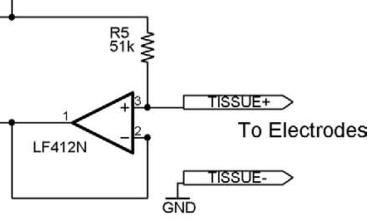
\includegraphics[width=6cm]
{Figure/elektroderdia}}
\caption{Der blev målt over elektroderne mellem ben 3 på LF412N og ground.}
\label{fig:elektroderdia}
\end{figure}

\section{Software}
\subsection{Waveforms}

I programmet Waveforms (som styrer Analog Discovery) kan frekvens og amplitude indstilles og resultatet kan ses i oscilloskopet. Dette blev brugt som det første til at måle og se om der kunne detekteres et synk.

\begin{figure}[H]
\centering
{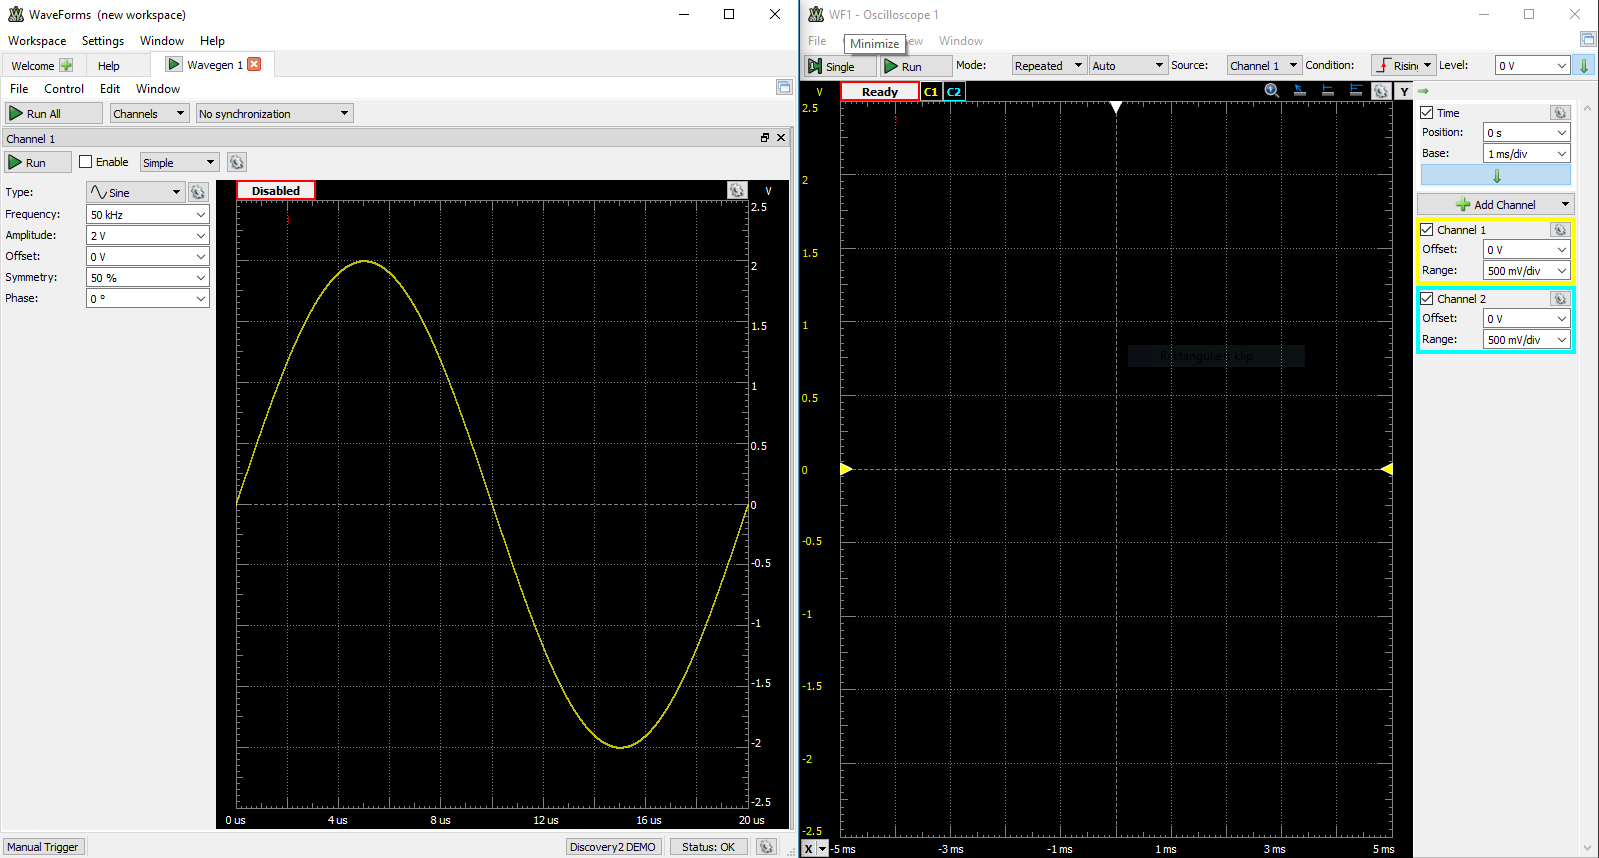
\includegraphics[width=14cm]
{Figure/waveforms}}
\caption{Brugerinterfacet i Waveforms, hvor funktionsgeneratoren og oscilloskop indstilles. }
\label{fig:waveforms}
\end{figure}











\section{Test af BI-måler}

Nu vil kredsløbet blive testet. Kredsløbet blev bygget i simuleringsprogrammet multisim og på et fumlebræt. Begge med samme udgangspunkt som i figur \ref{fig:testopstilling1}. I den kommende testopstilling vil der blive bekræftet systemtes virkning op i mod dokumentationen fra den oprindelige artikel og andre testmetoder fra andre artikler. Da de i den oprindelige artikel brugte kredsløbet til at måle på skalpen vil der ske løbende ændringer af kredsløbet som passer bedre til at måle et synk over svælget med inspiration fra andre artikler. 





I testopstillingen blev kredsløbet bygget efter figuer \ref{fig:testopstilling1} først i multisim og bagefter på et fumlebræt. Testen og resultaterne blev holdt op i mod dokumentationen fra den oprindelige artikel, som kan ses i figur \ref{fig:oprindeligeonload} og \ref{fig:oprindeligerms}. Ved at sammenligne resultaterne var det muligt at se om kredsløbet opførte sig korrekt og om det kunne bruges i den videre udvikling af synkerefleksmonitor. 

\begin{figure}[H]
\centering
{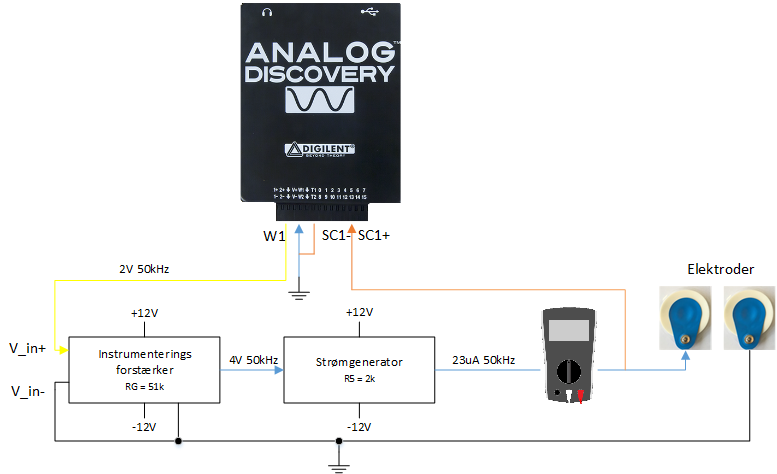
\includegraphics[width=\linewidth]
{Figure/testopstilling11}}
\caption{Diagram over testopstilling  på baggrund af det oprindelige kredsløbsdesign.}
\label{fig:testopstilling1}
\end{figure}

I artiklen får de grafen som vist i \ref{fig:oprindeligeonload} fra deres kredsløb ved at der ikke er noget load på udgangen. Den fortæller hvad strømmen er ved forskellige frekvenser og at den er stabil fra 1 kHz til 100 kHz. 

\begin{figure}[H]
\centering
{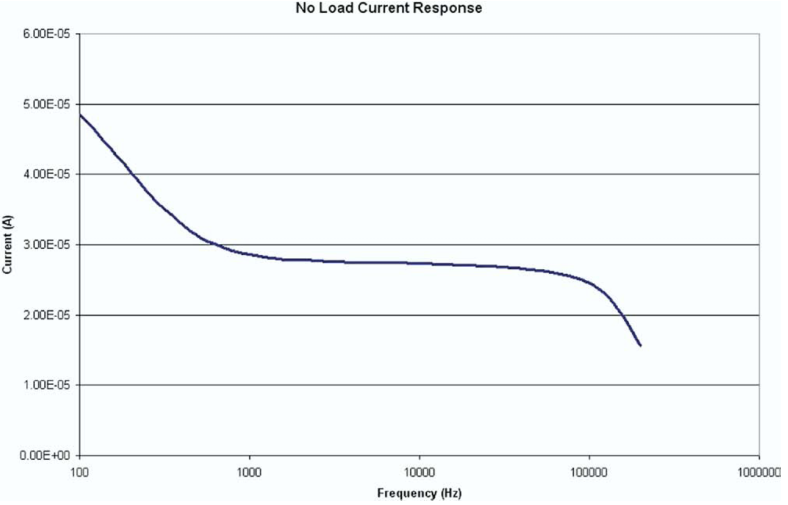
\includegraphics[width=10cm]
{Figure/oprindeligenoload}}
\caption{No-Load strøm respons af VCCS fra den oprindelige artikel\cite{Aroom2009}.}
\label{fig:oprindeligeonload}
\end{figure}

Grafen i figur \ref{fig:oprindeligerms} viser spændingen ændre sig ved forskellige frekvenser når der er påsat en vævsmodel på udgangen af kredsløbet hvor elektroderne skal sidde. 


\begin{figure}[H]
\centering
{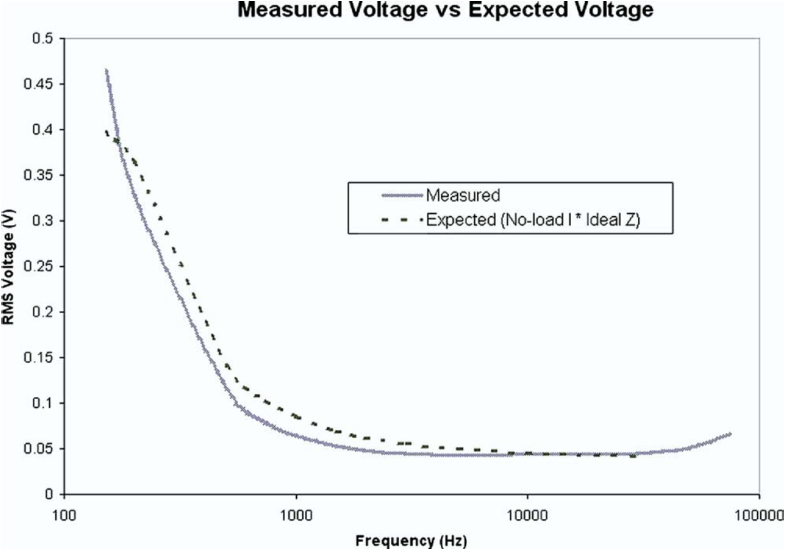
\includegraphics[width=10cm]
{Figure/oprindeligerms}}
\caption{Målte spændinger over elektroderne med en vævsmodel påsat  fra den oprindelige artikel\citep{Aroom2009}.}
\label{fig:oprindeligerms}
\end{figure}

\subsection{Simulering}

Opstiling af simuleringen af testopstilling kan ses i figur \ref{fig:testopstilling1multisim}. 

\begin{figure}[H]
\centering
{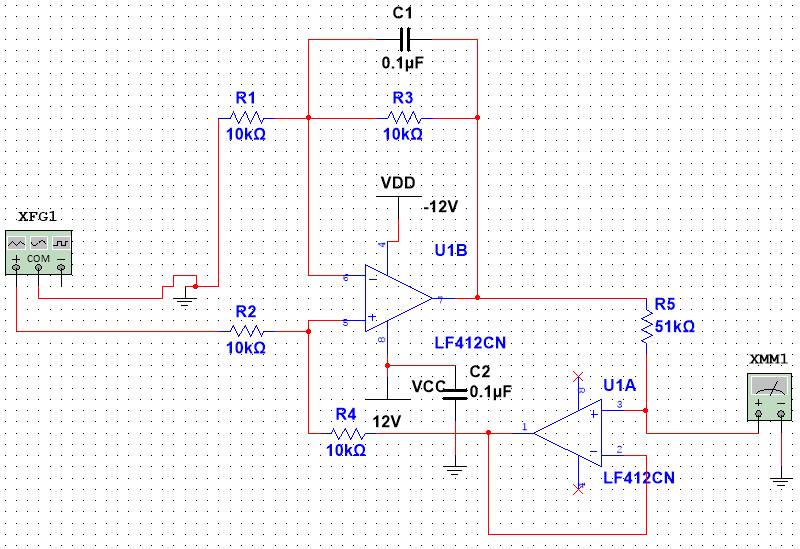
\includegraphics[width=10cm]
{Figure/testopstilling1multisim}}
\caption{Diagram over testopstilling i multisim på baggrund af det oprindelige kredsløbsdesign, dog uden instrumentationsforstærker.}
\label{fig:testopstilling1multisim}
\end{figure}

\subsubsection{No-Load}
\textbf{No-Load}\\
Til at bekræfte No-Load responset blev funktionsgeneratoren sat til 4V og 100Hz. På udgangen sad amperemeter for at kunne aflæse den konstante strøm.

Det kunne nu måles at den konstante strøm er på 49uA ved 100Hz, som det fremgår af figur \ref{fig:testopstilling1multisimnoload} hvilket stemmer fint overens med figur \ref{fig:oprindeligeonload} fra den oprindelige artikel. Ved at foretage flere målinger ved at variere frekvensen kan der tegnes en graf til sammenligning.

\begin{figure}[H]
\centering
{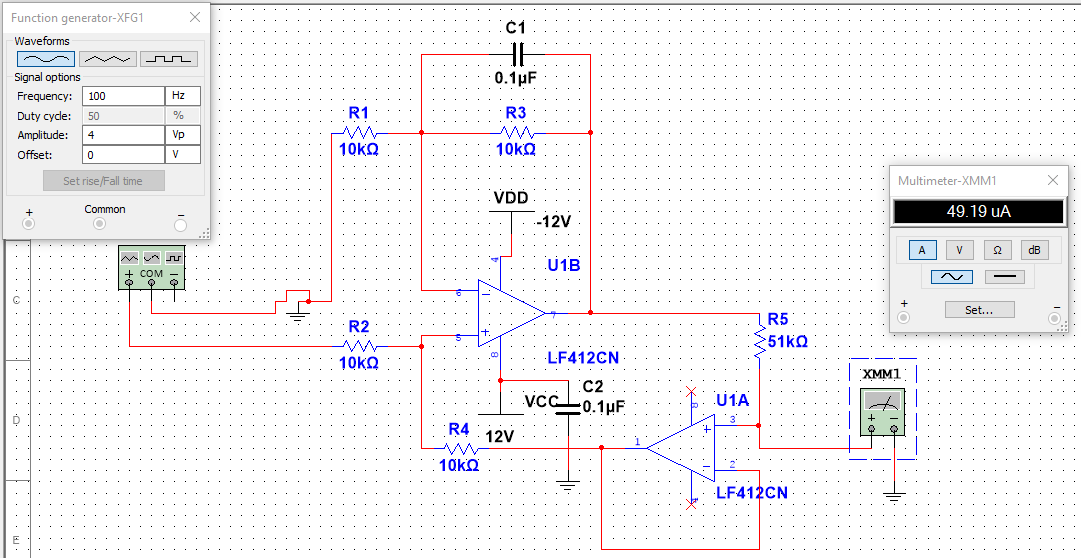
\includegraphics[width=10cm]
{Figure/testopstilling1multisimnoload}}
\caption{Diagram over testopstilling 1 i multisim ved 4 V og 100 Hz, kan den konstante strøm aflæses til 49uA.}
\label{fig:testopstilling1multisimnoload}
\end{figure}

I tabel \ref{table:frekvensernoload} kan de brugte frekvenser ses og går fra 100 Hz til 1 MHz med et passende interval. På baggrund af disse målinger kan der laves en graf over strøm responset som i \ref{fig:oprindeligeonload}.

\begin{table}[H]
\centering
\begin{tabular}{| r | r || r | r || r | r || r | r |}
    \hline
    \textbf{Hz} & \textbf{uA} & \textbf{Hz} & \textbf{uA} & \textbf{Hz} & \textbf{uA} & \textbf{Hz} & \textbf{uA}\\ \hline
    100 & 49,19 & 2000 & 27,99 & 30000 & 27,73 & 400000 & 27,87  \\ \hline
    200 & 40,74 & 3000 & 27,84 & 40000 & 27,73 & 500000 & 27,93  \\ \hline
    300 & 35,68 & 4000 & 27,79 & 50000 & 27,73 & 600000 & 27,99  \\ \hline
    400 & 32,90 & 5000 & 27,77 & 60000 & 27,73 & 700000 & 28,07  \\ \hline
    500 & 31,30 & 6000 & 27,76 & 70000 & 27,74 & 800000 & 28,16  \\ \hline
    600 & 30,32 & 7000 & 27,75 & 80000 & 27,74 & 900000 & 28,25  \\ \hline
    700 & 29,69 & 8000 & 27,75 & 90000 & 27,74 & 1000000 & 28,32  \\ \hline
    800 & 29,26 & 9000 & 27,74 & 100000 & 27,74 &  &   \\ \hline
    900 & 28,95 & 10000 & 27,74 & 200000 & 27,78 &  &   \\ \hline
    1000 & 28,73 & 20000 & 27,73 & 300000 & 27,82 &  &  \\ \hline
\end{tabular}
    \caption{Målt strøm over elektroderne ved bestemte frekvenser.}
    \label{table:frekvensernoload}
\end{table} 


\begin{figure}[H]
\centering
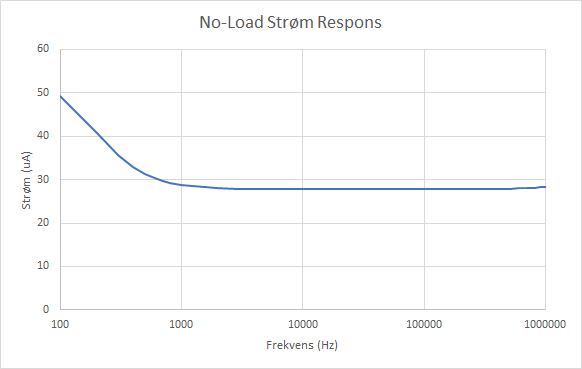
\includegraphics[width=10cm]{Figure/testopstilling1multisimnoloadgraf}
\captionof{figure}{Resultatet af den målte strøm ved varieret frekvenser, som kan sammenlignes med figur \ref{fig:oprindeligeonload}. X aksen er i logaritmisk skala.}
\label{fig:testopstilling1multisimnoloadgraf}
\end{figure}


\subsubsection{RMS spænding}

Den målte spænding måles over elektroderne og ved at tilføje en vævsmodel som i figur \ref{fig:testopstilling1multisimvaevs}, vil spændingen ændre sig ved forskellige frekvenser. Vævsmodellen bruges til at vertificere nøjeagtighed og repeterbarhed af kredsløbet\cite{Aroom2009}.

\begin{figure}[H]
\centering
{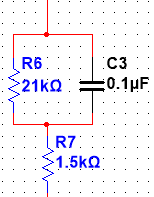
\includegraphics[width=4cm]
{Figure/testopstilling1multisimvaevs}}
\caption{Vævsmodel med to modstande og en kondensator, som viser en elektrisk model over et væv.}
\label{fig:testopstilling1multisimvaevs}
\end{figure}




\begin{figure}[H]
\centering
{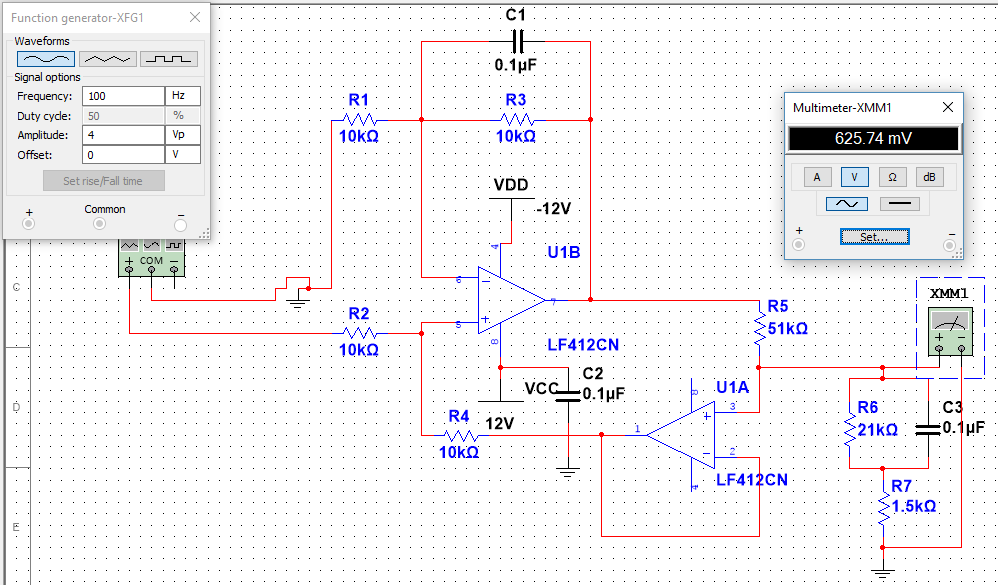
\includegraphics[width=10cm]
{Figure/testopstilling1multisimRMS}}
\caption{Diagram over testopstilling i multisim ved 4V og 100Hz, hvor spændingen kan aflæses over vævsmodellen.}
\label{fig:testopstilling1multisimRMS}
\end{figure}

De målte spændinger som vist i tabel \ref{table:frekvenservrms} er målt fra 100 Hz til 100 kHz.  Målingerne får følgende graf vist i figur \ref{fig:testopstilling1multisimVRMSgraf} 

\begin{table}[H]
\centering
\begin{tabular}{| r | r || r | r || r | r |}
    \hline
    \textbf{Hz} & \textbf{VRMS} & \textbf{Hz} & \textbf{VRMS} & \textbf{Hz} & \textbf{VRMS}\\ \hline
    100 & 0,626 & 2000 & 0,047 & 30000 & 0,041 \\ \hline
    200 & 0,311 & 3000 & 0,044 & 40000 & 0,041   \\ \hline
    300 & 0,195 & 4000 & 0,043 & 50000 & 0,041   \\ \hline
    400 & 0,141 & 5000 & 0,042 & 60000 & 0,041   \\ \hline
    500 & 0,112 & 6000 & 0,042 & 70000 & 0,041  \\ \hline
    600 & 0,094 & 7000 & 0,042 & 80000 & 0,041   \\ \hline
    700 & 0,083 & 8000 & 0,041 & 90000 & 0,041  \\ \hline
    800 & 0,074 & 9000 & 0,041 & 100000 & 0,041   \\ \hline
    900 & 0,068 & 10000 & 0,041 &  &     \\ \hline
    1000 & 0,064 & 20000 & 0,041 & &   \\ \hline
\end{tabular}
    \caption{Målt VRMS ved bestemte frekvenser.}
    \label{table:frekvenservrms}
\end{table} 


\begin{figure}[H]
\centering
{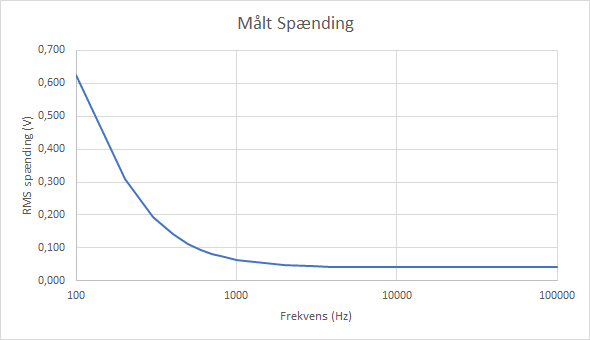
\includegraphics[width=10cm]
{Figure/testopstilling1multisimVRMSgraf}}
\caption{Grafen viser de plottet frekvenser, som kan sammenlignes med figur \ref{fig:oprindeligerms} fra den oprindelige artikel.}
\label{fig:testopstilling1multisimVRMSgraf}
\end{figure}








\subsection{Fumlebræt}

Der blev foretaget samme målinger på fumlebræt. Opstillingen af fumlebrættet kan ses i figur \ref{fig:oprindeligekredslob2}. Den øverst bane var +12V (rød), den nederste bane var -12 V (grøn) og stel sort.  


\begin{figure}[H]
\centering
{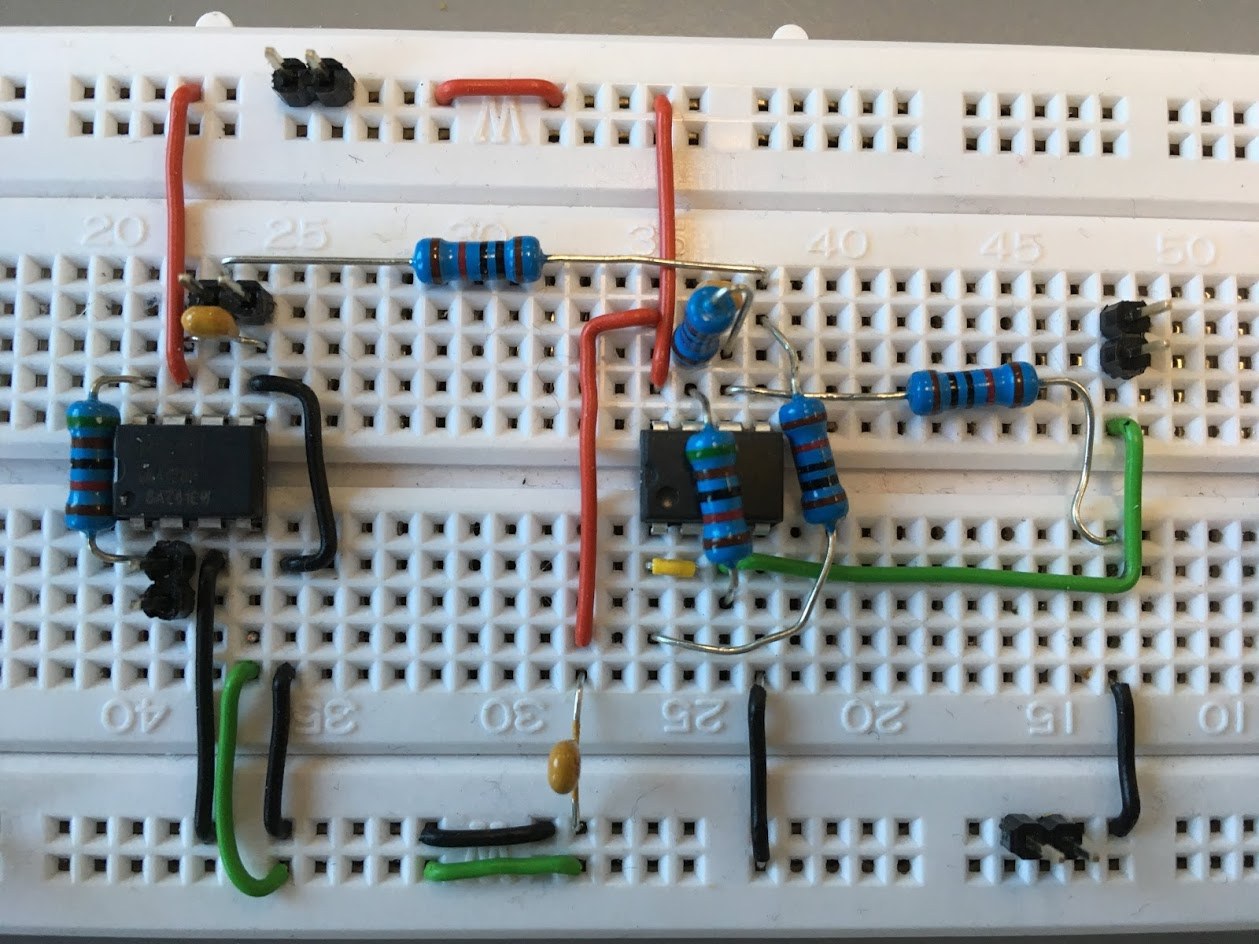
\includegraphics[width=8cm]
{Figure/oprindeligekredslob2}}
\caption{Billede af testopstilling på fumlebræt på baggrund af det oprindelige kredsløbsdesign. INA128 til venstre og LF412CN til højre.}
\label{fig:oprindeligekredslob2}
\end{figure}


\subsubsection{No-Load}
Der blev udført no-load test fra 100 Hz til 220 kHz og strømmen blev aflæst. Resultatet af de målte værdier kan ses i tabel \ref{table:frekvensernoload2}, efterfølgende blev der lavet en graf af resultaterne som kan ses i figur \ref{fig:testopstilling1fumlenoloadgraf}.


\begin{figure}[H]
\centering
{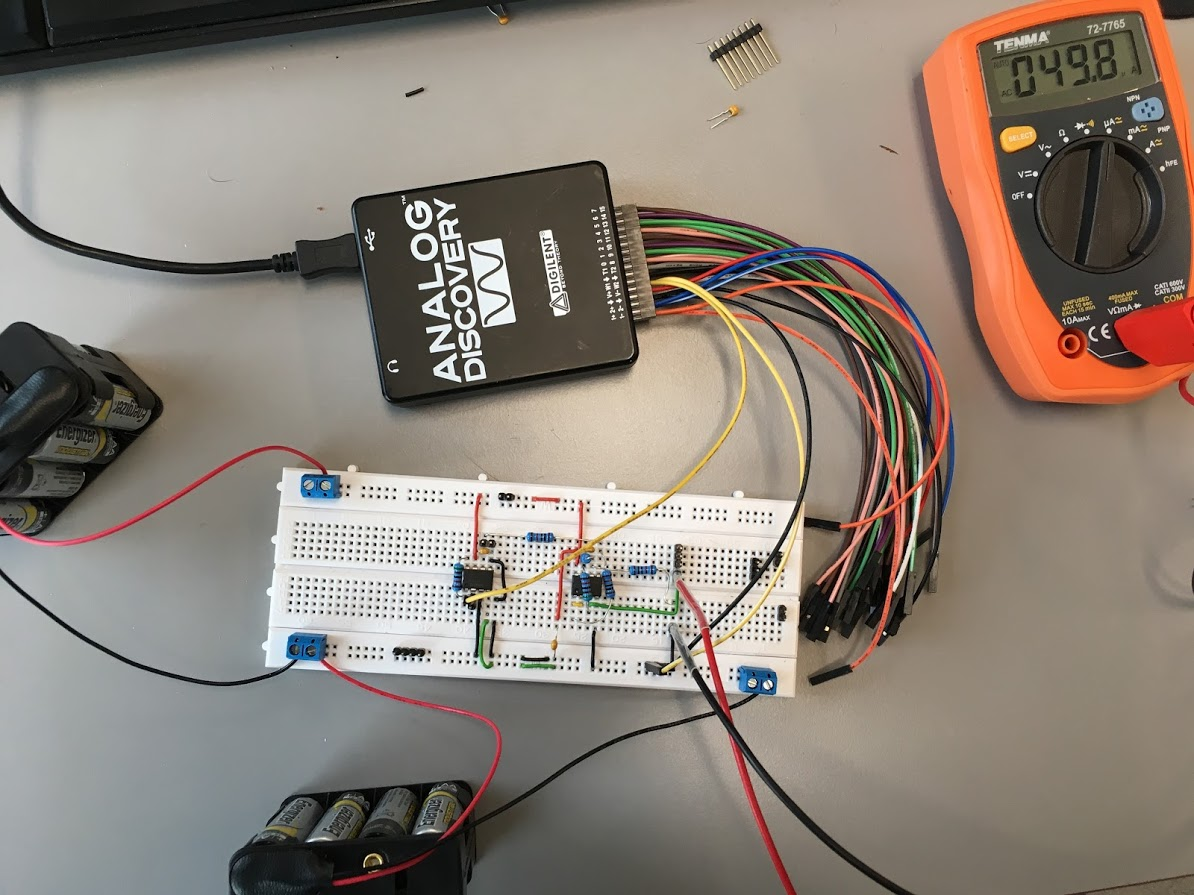
\includegraphics[width=8cm]
{Figure/oprindeligekredslobfumle1}}
\caption{Billede af testopstilling på fumlebræt ved 100 Hz og en konstant strøm på 49 uA.}
\label{fig:oprindeligekredslobfumle1}
\end{figure}





\begin{table}[H]
\centering
\begin{tabular}{| r | r || r | r || r | r || r | r |}
    \hline
    \textbf{Hz} & \textbf{uA} & \textbf{Hz} & \textbf{uA} & \textbf{Hz} & \textbf{uA} & \textbf{Hz} & \textbf{uA}\\ \hline
    100 & 49,8 & 2000 & 28,1 & 30000 & 25 & 130000 & 23,9  \\ \hline
    200 & 41,5 & 3000 & 27,8 & 40000 & 24,1 & 140000 & 24,3  \\ \hline
    300 & 36,5 & 4000 & 27,6 & 50000 & 23,2 & 150000 & 23,8  \\ \hline
    400 & 33,6 & 5000 & 27,5 & 60000 & 22,5 & 160000 & 20,7  \\ \hline
    500 & 31,9 & 6000 & 27,4 & 70000 & 21,2 & 170000 & 3,2  \\ \hline
    600 & 30,8 & 7000 & 27,3 & 80000 & 20,2 & 180000 & 1,1  \\ \hline
    700 & 30,2 & 8000 & 27,2 & 90000 & 20,6 & 190000 & 0,5  \\ \hline
    800 & 29,3 & 9000 & 27 & 100000 & 21,4 &  200000 & 0,3  \\ \hline
    900 & 29,3 & 10000 & 26,9 & 110000 & 22,3 &  210000 & 0,2   \\ \hline
    1000 & 29,1 & 20000 & 25,9 & 120000 & 23,2 &  220000 & 0,1  \\ \hline
\end{tabular}
    \caption{Målt strøm over elektroderne ved bestemte frekvenser.}
    \label{table:frekvensernoload2}
\end{table} 



\begin{figure}[H]
\centering
{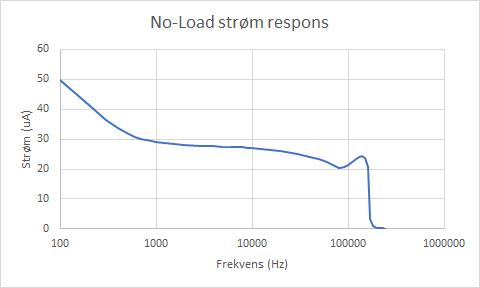
\includegraphics[width=10cm]
{Figure/testopstilling1fumlenoloadgraf}}
\caption{Grafen viser målt RMS.}
\label{fig:testopstilling1fumlenoloadgraf}
\end{figure}


\subsubsection{RMS spænding}
Ved at tilføre vævsmodellen som i figur \ref{fig:testopstilling1fumlevaevs} kunne spændingerne måles.


\begin{figure}[H]
\centering
{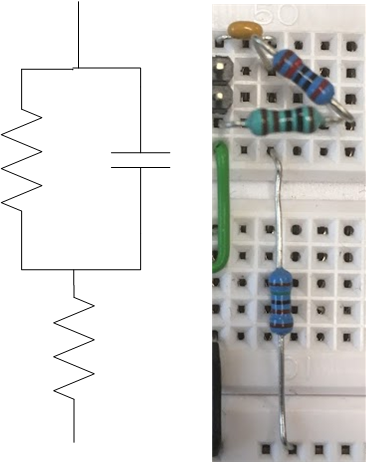
\includegraphics[width=8cm]
{Figure/testopstilling1fumlevaevs}}
\caption{I vævsmodellen er der brugt modstande på 20 kohm, 1 kohm (i serie) og 1,5 kohm. Kondensatoren var på 0,1 uF.}
\label{fig:testopstilling1fumlevaevs}
\end{figure}

Frekvensen blev varieret fra 100 Hz til 100 kHz og RMS spændningerne blev aflæst og resultatet kan ses i tabel \ref{table:fumlebraetfrekvenservrms}. På baggrund af målingerne blev kunne disse blive tegnet i en graf som kan ses i figur \ref{fig:testopstilling1fumlevrmsgraf} til sammenligningsgrundlag med de tidligere VRMS grafer.

\begin{table}[H]
\centering
\begin{tabular}{| r | r || r | r || r | r |}
    \hline
    \textbf{Hz} & \textbf{VRMS} & \textbf{Hz} & \textbf{VRMS} & \textbf{Hz} & \textbf{VRMS}\\ \hline
    100 & 0,6375 & 2000 & 0,068 & 30000 & 0,0502 \\ \hline
    200 & 0,3294 & 3000 & 0,062 & 40000 & 0,0504   \\ \hline
    300 & 0,2132 & 4000 & 0,058 & 50000 & 0,0501   \\ \hline
    400 & 0,1593 & 5000 & 0,054 & 60000 & 0,0505   \\ \hline
    500 & 0,13 & 6000 & 0,052 & 70000 & 0,0512  \\ \hline
    600 & 0,1129 & 7000 & 0,0513 & 80000 & 0,0507   \\ \hline
    700 & 0,1015 & 8000 & 0,051 & 90000 & 0,0514  \\ \hline
    800 & 0,09345 & 9000 & 0,0507 & 100000 & 0,0507   \\ \hline
    900 & 0,08805 & 10000 & 0,0515 &  &     \\ \hline
    1000 & 0,084 & 20000 & 0,0502 & &   \\ \hline
\end{tabular}
    \caption{Målt VRMS ved bestemte frekvenser på fumlebræt.}
    \label{table:fumlebraetfrekvenservrms}
\end{table} 


\begin{figure}[H]
\centering
{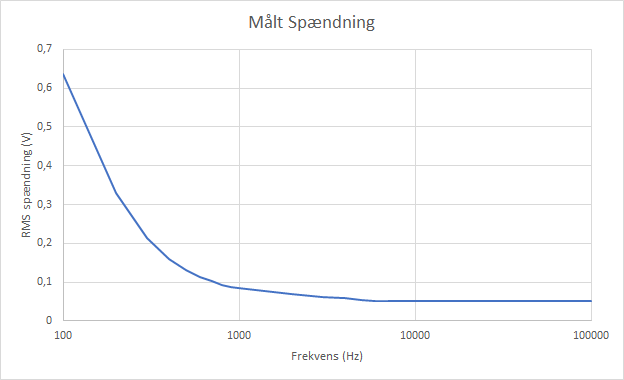
\includegraphics[width=10cm]
{Figure/testopstilling1fumlevrmsgraf}}
\caption{Grafen viser de målte VRMS fra 100 Hz til 100 kHz.}
\label{fig:testopstilling1fumlevrmsgraf}
\end{figure}

\section{Detektion af synk}

Detektionen af synk vil foregå med fumlebrættet. Først med en variable modstand efterfølgende med elektroder påsat som load. Ved den variable load modstand kan det ses i figur \ref{fig:10kohmdummysynk}, at et synk kan vises ved at dalene i signalet er når modstanden bliver mindre og går så op igen når modstanden øges. Dette er en meget forsimplet test og der er ikke taget højde for sampling, filtering m.m. Strømmen var stabil imellem 23 uA og 20 uA.

\begin{figure}[H]
\centering
{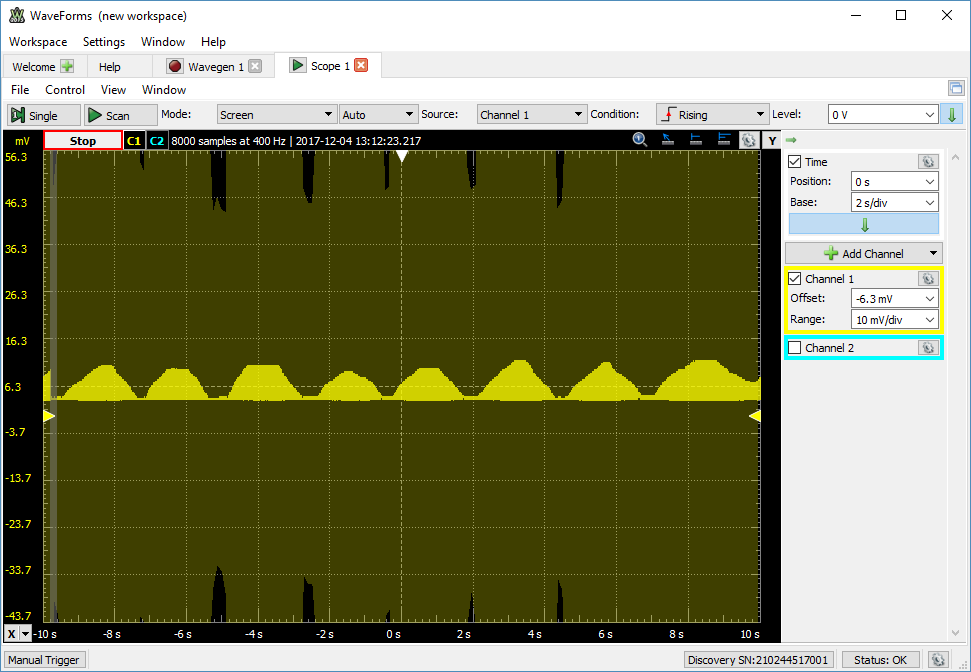
\includegraphics[width=10cm]
{Figure/10kohmdummysynk}}
\caption{Simuleret et synk på fumlebræt ved at montere en variable 10 kohm som load modstand. Dette er ved 50 kHz og med en amplitude på 2 V fra Analog Discovery.}
\label{fig:10kohmdummysynk}
\end{figure}


Det målte signal i figur \ref{fig:synk1} viser en måling med elektroder og hvor der er foretaget synk. Det der blev kigget efter i målingen var om der kom et spændingsfald når der blev foretaget et synk. Det var ikke muligt at se nogen ændring i spændingsfaldet ved at se om signalet blev fladere. 

\begin{figure}[H]
\centering
{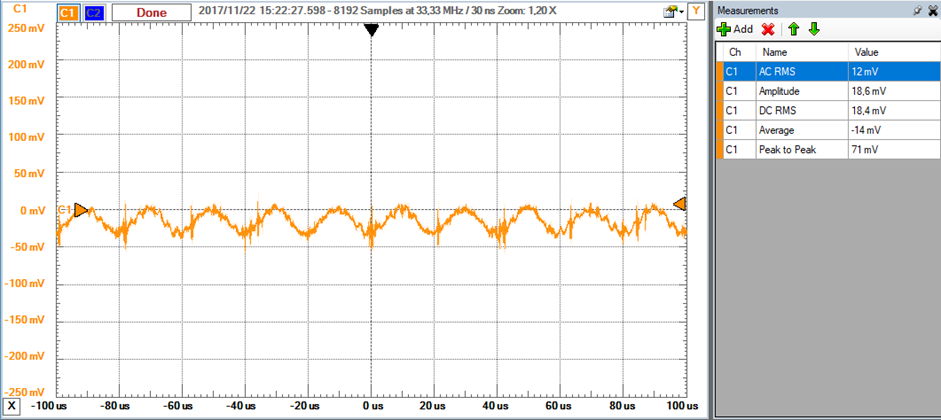
\includegraphics[width=10cm]
{Figure/synk1}}
\caption{Målt synk med påsatte elektroder. Dette er ved 50 kHz og amplitude på 2 V.}
\label{fig:synk1}
\end{figure}








\chapter{EMG-måler}

Udover BI-måleren vil der blive brugt en kommercielt EMG-måler som i figur \ref{fig:emgdata}, MyoWare Muscle Sensor til at detektere synk. Da BI-måleren ikke kan stå alene om at detektere et synk er det muligt at tilføje en EMG-måler der måler muskelaktiviteten ved svælget. 

\begin{figure}[H]
\centering
{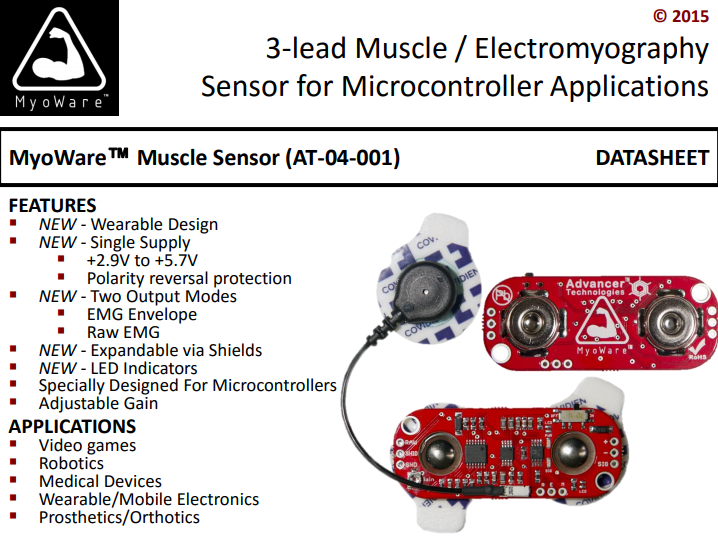
\includegraphics[width=10cm]
{Figure/emgdata}}
\caption{Overblik over EMG-måleren fra databladet.}
\label{fig:emgdata}
\end{figure}

Den vil få sine egne elektroder og der er brug for tre styk. Samplingen vil ske ved hjælp af Analog Discovery. Den vil blive forsynet med egen spændingskilde på 4,5 V. Der vil i første omgang blive brugt udgangen "EMG Envelope" da det ikke vil kræve yderligere filtrering eller databehandling.
 



\chapter{Konklusion}

Ved først at simulere og bagefter bygge kredsløbet i artiklen har været meget lærerigt. Det gav en ide om hvad en BI-måler skal kunne og indeholde. Dette vil være udgangspunktet for udviklingen af Synkerefleksmonitor.  

Test resultaterne af no-load og Vrms ligner meget lig de resultater fra artiklen. Det har ikke været muligt at bruge præcis samme udstyr, men kredsløbet er identisk hvilket må være acceptabelt.

For at udvikle Synkerefleksmonitor der kritiske ting som skal tilføjes og ændres fra det oprindelige kredsløb:
\begin{itemize}
\item Større strøm
\item 4 elektroder
\item Filtrering
\item A/D konvertering
\end{itemize}

Strømmen der bliver ført over i måleobjektet skal være større, da det er kendt at den ligger ved 500 uA\cite{Kusuhara2004} når der skal måles over svælget og ikke på skalpen som er tilfældet i artiklen. Dette vil kræve en udvikling af en ny VCCS med udgangspunkt i howland som fra artiklen.

Når der måles BI bliver dette typisk gjort ved hjælp af fire elektroder\cite{Brantlov2017}. To til at overføre strømmen og to til at måle spændingsfaldet med. To elektroder vil også kunne skabe impedans inteferanse i elektroderne hvilket kan resulterer i fejlmålinger. Dette kræver en opdeling af et strømkredsløb med howland og et som måler spændningen fra måleobjektet.

I artiklen bliver der ikke omtalt filterring af det samplet signal. Dette vil blive et must da for at undgå antialisering\cite{Thomas2011} skal dette udvikles til systemet.


En kritisk del af synkerefleksmonitor er dataopsamlingen. For at begrænse A/D konvertere til et minimum vælges Analog discovery til at både at fungere som funktionsgenerator og sample signalet. Det skaber dog en begrænsning i hvor hurtigt Analog Discovery da den nu skal sample to signaler (BI-måler og EMG-måler simultant), hvilket resulterer i at det er nødvendigt at reducere samplingsfrekvens. Udover at samplingsfrekvensen skal sættes ned, er det også nødvendigt at nedsætte de 50 kHz. Det vil sige at Analog Discovery kan maks. sample ved 500 kHz når der skal bruge to analog kanaler. Dette gør at for at få en korrekt databehandling og den videre udvikling af synkerefleksmonitor nedsættes funktionsgeneratoren til 20 kHz.

Et overblik over de nye tiltag i forhold til artikel kredløbet kan ses i figur \ref{fig:konklusiondiagram}. 



\begin{figure}[H]
\centering
{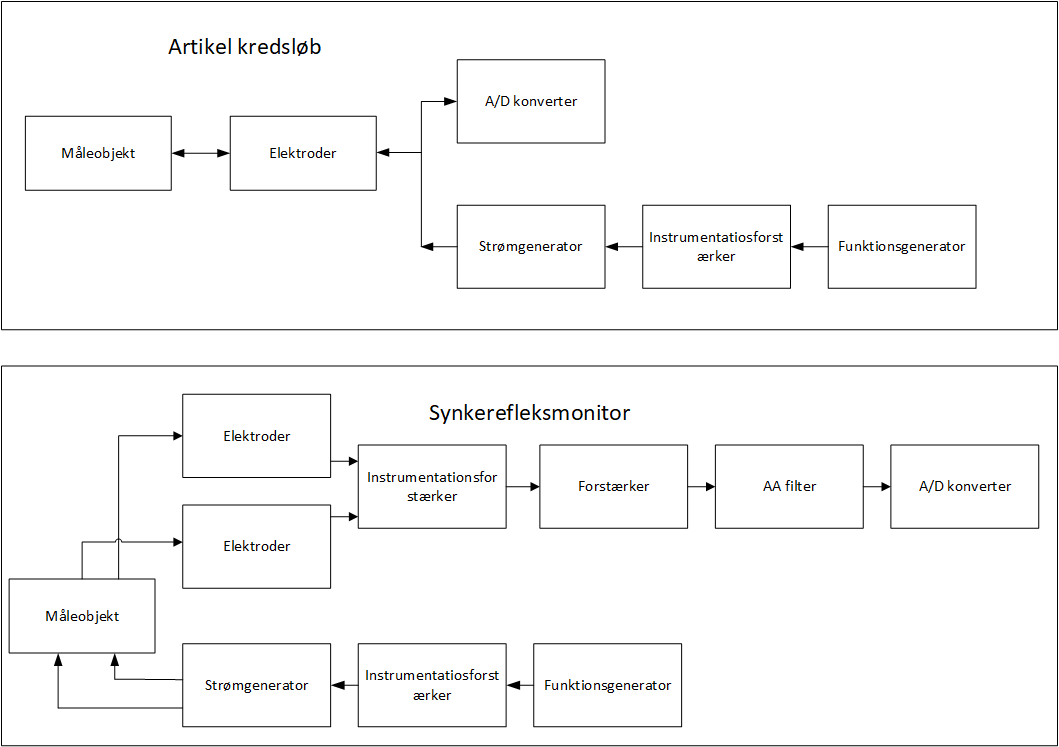
\includegraphics[width=\linewidth]
{Figure/konklusiondiagram}}
\caption{Øverst er det simple kredsløb fra artiklen. Nederst er det ønsket mere komplekse Synkerefleksmonitor.}
\label{fig:konklusiondiagram}
\end{figure}




%\chapter{Det modificeret kredsløb}
%Erfaringerne fra det oprindelige kredsløb og metoder fra andre artikler blev testet for til slut at kunne vælge det endelige videre system i projektet. Den overordnet ændring er at hardware blev delt op i to dele, en strømgenerator og spændingsmåler. Denne løsning er blevet brugt i flere artikler, \cite{Nahrstaedt2012a}, \cite{Chester}.





%\section{Hardware del 1 - Strømgenerator}

%I denne hardware del 1 blev der genereret strøm til to elektroder. I figur \ref{fig:analyse1} kan de enkelte komponenter ses.


%\begin{figure}[H]
%\centering
%{\includegraphics[width=\linewidth]
%{Figure/analyse1}}
%\caption{Forløbet over generationen af den faste strøm.}
%\label{analyse1}
%\end{figure}

%\subsection{Strømforsyning}
%Strømforsyningen er blevet øget fra $\pm$12 til $\pm$18 da dette giver en højere excitationsspænding som bidrager til en øget strøm som kan genereres.
%\begin{figure}[H]
%\centering
%{\includegraphics[width=8cm]
%{Figure/18v}}
%\caption{Ved brug af fire 9V batterier kan excitationsspænding komme op på $\pm$18V.}
%\label{fig:18v}
%\end{figure}
%
%\subsection{Funktionsgenerator}
%Signalet fra funktionsgeneratoren blev øget til 4V og bibeholdt 50kHz.
%\subsection{Forstærkning}
%Forstærkningen blev nu øget fra 4V til 8V strømgeneratoren.
%
%\subsection{Strømgenerator}
%Der vælges at øge strømmen til 500uA ved at ændre R5 til 2k, da artiklerne \cite{Chester}, \cite{Chester2014} og \cite{Kusuhara2004} bruger denne strøm til at detektere BI over svælget. 
%
%
%
%
%
%\subsection{Elektroder}
%
%Der blev testet med begge elektroder fra figur \ref{fig:elektroder} og med forskellige placeringer. Strømmen og den målte spændingen er nu blevet ført over sine egne ledninger. BI er bedst at måle med fire elektroder, for at undgå utilsigtet inklusion af elektrode impedans ved kun brug af to elektroder \cite[s. 420-421]{Holder2004}.
%
%
%\begin{figure}[H]
%\centering
%{\includegraphics[width=8cm]
%{Figure/elektrodeplacering1}}
%\caption{Der er prøvet med forskellige elektrode placeringer. Hvor strøm elektroder er yderst og spændingen måles inderst.}
%\label{fig:elektroder2}
%\end{figure}
%
%
%
%\begin{figure}[H]
%\centering
%{\includegraphics[width=8cm]
%{Figure/BIbasic}}
%\caption{Diagram for hvordan man måler BI, med en fast strøm hvor spændingen kan måles over.}
%\label{fig:analyse2}
%\end{figure}
%
%
%\section{Hardware del 2 - Spændingsmåler}
%\begin{figure}[H]
%\centering
%{\includegraphics[width=\linewidth]
%{Figure/analyse2}}
%\caption{Bioimpedans ud}
%\label{fig:analyse2}
%\end{figure}
%
%
%\subsection{Strømforsyning}
%
%Da strømforsyningen var øget til $\pm$18V for del 1, blev del 2 forsynet med den samme excitationsspænding. 
%
%\subsection{Elektroder}
%
%Der blev testet med begge elektroder fra figur \ref{fig:elektroder} og med forskellige placeringer.
%
%\subsection{Forstærkning}
%Da det var en lille spænding der måltes blev den forstærket op samtidig med at støj blev reduceret. Der blev stadig holdt øje om båndbredden var indenfor hvad INA128 kunne leverer ved forskellige gains. Gain blev sat til 10, hvilket der ok som det kan aflæses i figur \ref{fig:ina128gain}.
%
%
%\subsection{Antialiaseringsfilter}
%Antialiaseringsfilteret består af et lavpas filter med en knækfrekvens på 50kHz, da synket er blevet amplitudemoduleret ved denne frekvens. Lavpasfilteret blev et 2.ordenfilter da det ville dæmpe med -40dB pr. dekade, således at ved 500kHz er det dæmpet -40dB.
%
%
%
%\subsection{A/D konverter}
%Når signalet er blevet forstærket til det ønskede spændingsniveau som er brugbart for A/D konverteren, er det muligt at sample signalet. Ved at vælge en høj samplingfrekvens på 1MHZ, fik vi samplet det dobbelte af det halve af nyquist frekvens.
%
%\section{Software}
%\subsection{Matlab}
%
%\section{Testopstillinger}
%\subsection{Testopstilling 1}
%\subsection{Testopstilling 2 - LM318N}
%\subsection{Testopstilling 3 - OPAMP}
%\begin{figure}[H]
%\centering
%{\includegraphics[width=\linewidth]
%{Figure/modificeretkredslob}}
%\caption{}
%\label{modificeretkredslob}
%\end{figure}
%
%\section{Konklusion}
%
%\chapter{EMG}
%
%
%
%
%
%
%\begin{figure}[H]
%\centering
%{\includegraphics[width=\linewidth]
%{Figure/analyse1}}
%\caption{Bioimpedans ud}
%\label{fig:analyse1}
%\end{figure}
%
%Instrumenterings forstærker 1\\
%I det oprindelig design af BI konstateret vi at det var lavet lavet til at måle BI'er på skalpen og ikke over svælget. Derfor valgte vi at instrumenterings forstærkeren fik et større signal ind fra Analog Discovery på 2V og 50kHz. I det hele taget undrede vi over artiklens valg af brug af instrumenterings forstærker i starten af kredsløbet, da den ikke er et must for at realisere kredsløbet. Men dens eneste formål var at nedbringe common-mode støj fra funktions generatoren, så vi valgte at beholde denne da vi også vil undgå så meget støj som muligt videre i kredsløbet. Gain var oprindeligt sat til 51 Kohm hvilket giver det dobbelte af hvad instrumenterings forstærkeren tilføre. I diagrammet på figur \ref{BIdiagram} kan det ses at instrumenterings forstærkeren bliver forsynet med +12/-12 V, men der er her valgt at -12 V skal direkte til ground, hvilket har resulteret i at instrumenterings forstærkeren ikke fungerer korrekt, så der er den i stedet forsynet med -12 V og ikke ground.  
%
%
%
%
%
%Strømgenerator\\
%Det forstærket signal som kommer fra udgangen på instrumenterings forstærkeren løber over til strømgeneratoren. Denne strømgenerator er en Howland bridge. Sammensætningen af modstandene er vigtige og deres tolerance skal være lav for at få en korrekt og konstant strøm. For at justerer strømmen kan R5 udskiftes i kredsløbet. For at få en konstant strøm omkring ca. 500 uA, er modstanden ændret fra 51 Kohm til 2 Kohm.  
%
%\textbf{Det oprindelige kredsløb}\\
%Først bygges det oprindelige kredsløb som det er opgivet og der bliver foretaget en no load test, for at se om det stemmer overens med figuren fra artiklen.
%
%\begin{figure}[H]
%\centering
%\begin{minipage}{.5\textwidth}
%  \centering
%  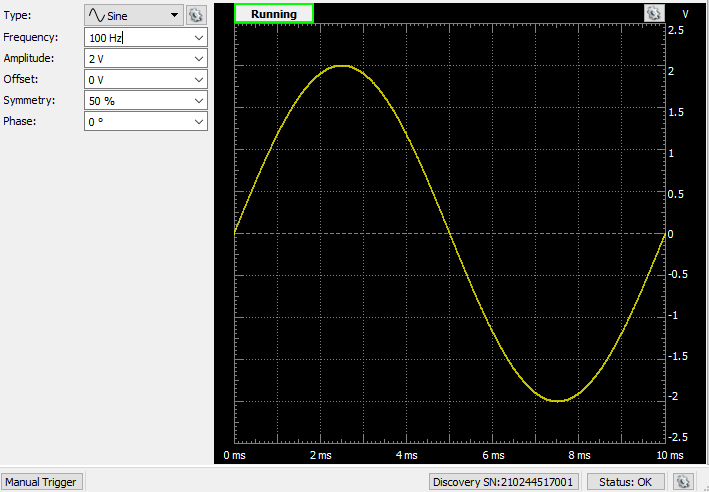
\includegraphics[width=.9\linewidth]{Figure/VCCSwavegen1}
%  \captionof{figure}{A figure}
%  \label{fig:test1}
%\end{minipage}%
%\begin{minipage}{.5\textwidth}
%  \centering
%  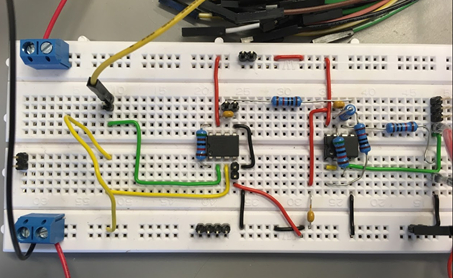
\includegraphics[width=.9\linewidth]{Figure/oprindeligekredslob}
%  \captionof{figure}{Another figure}
%  \label{fig:test2}
%\end{minipage}
%\end{figure}
%
%
%
%
%
%
%
%
%\textbf{Det modificeret kredsløb}\\
%
%\begin{table}[H]
%\begin{minipage}[b]{0.30\linewidth}
%\centering
%\begin{tabular}{ r |  r }
%    \hline
%    Hz & uA \\ \hline
%    100 & 1268 \\ \hline
%    200 & 1051 \\ \hline
%    300 & 920 \\ \hline
%    400 & 845 \\ \hline
%    500 & 802 \\ \hline
%    600 & 775 \\ \hline
%    700 & 756 \\ \hline
%    800 & 744 \\ \hline
%    900 & 735 \\ \hline
%    1000 & 728 \\ \hline
%    2000 & 703 \\ \hline
%    3000 & 696 \\ \hline
%    4000 & 692 \\ \hline
%    5000 & 688 \\ \hline
%    6000 & 685 \\ \hline
%    7000 & 683 \\ \hline
%    8000 & 680 \\ \hline
%    9000 & 678 \\ \hline
%    10000 & 676 \\ \hline
%    20000 & 675 \\ \hline
%    30000 & 634 \\ \hline
%    40000 & 596 \\ \hline
%    50000 & 542 \\ \hline
%    60000 & 475 \\ \hline
%    70000 & 405 \\ \hline
%    80000 & 332 \\ \hline
%    90000 & 268 \\ \hline
%    100000 & 210 \\ \hline
%    110000 & 161 \\ \hline
%    120000 & 120 \\ \hline
%    130000 & 87 \\ \hline
%    140000 & 60 \\ \hline
%    150000 & 40 \\ \hline
%    160000 & 25 \\ \hline
%    170000 & 16 \\ \hline
%    180000 & 10 \\ \hline
%    190000 & 6 \\ \hline
%    200000 & 4 \\ \hline
%    210000 & 2 \\ \hline
%    220000 & 1 \\ \hline
%    230000 & 1 \\ \hline
%    240000 & 0 \\ \hline
%        
%\end{tabular}
%    \caption{Student Database}
%    \label{table:student}
%\end{minipage}\hfill
%\begin{minipage}[b]{0.7\linewidth}
%\centering
%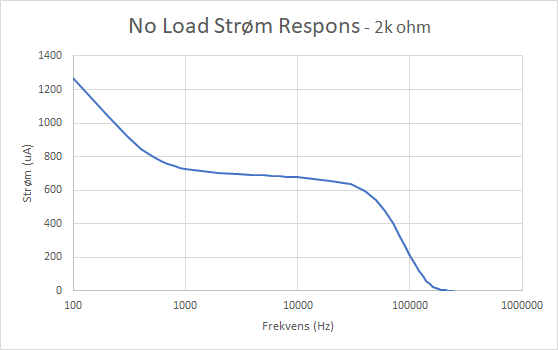
\includegraphics[width=10cm]{Figure/stromfrekvensoprindelig2k}
%\captionof{figure}{2-D scatterplot of the Student Database}
%\label{fig:image}
%\end{minipage}
%\end{table}
%
%
%
%
%
%
%
%
%
%
%
%
%
%
%Overvejelser om mulige løsninger
%løsninger I har valgt, begrundelsen herfor
%grundlæggende valg af hardware- og softwaremæssige komponenter, som er kritiske for realisering af systemet
%
%For at træffe et valg kan der analyseres og diskuteres forskellige løsninger mht. til ydeev-ne, pris, leveringstid og forhåndskendskab. Disse kan med fordel opstilles i tabelform.
%
%Anti-alisering
%Elektroder
%Konstant strøm
%Lavpas filtering
%Ensretter
%Sampling af signal 
%
%
%
%
%
%\chapter{Konklusion}
\bibliography{library}

\end{document}
